%Ich habe hie nur mal zu testzwecken einen sinnlosen Kommentar eingefuegt!
\documentclass[a4paper,10pt,notumble]{leaflet}
\usepackage[utf8]{inputenc}

\usepackage[scaled]{helvet}
\renewcommand\familydefault{\sfdefault} 
\usepackage[T1]{fontenc}
\usepackage[ngerman]{babel}
%\usepackage{setspace}
\usepackage{hyperref}
\usepackage{siunitx}
\sisetup{locale = DE}
\DeclareSIUnit[number-unit-product = { } ]
	\EUR{EUR}

\usepackage{graphicx}
\graphicspath{{gfx/}}

\newcommand{\meal}[4]{\textbf{#1}\hspace{3mm}%
\begin{minipage}[t]{5.5 cm}
\begin{flushleft}
#2\textsuperscript{#3}
\end{flushleft}
\end{minipage}%
\hfill\SI{#4}{\EUR}\newline}

% Allergen-Verzeichnis
\newcommand{\Getreideprodukte}{a}
\newcommand{\Fisch}{b}
\newcommand{\Krebstiere}{c}
\newcommand{\Schwefel}{d} 
\newcommand{\Sellerie}{e} 
\newcommand{\Laktose}{f} 
\newcommand{\Sesamsamen}{g} 
\newcommand{\Nuss}{h} 
\newcommand{\Eier}{i} 
\newcommand{\Lupinen}{j} 
\newcommand{\Senf}{k} 
\newcommand{\Soja}{l} 
\newcommand{\Weichtiere}{m} 
\newcommand{\Erdnuss}{n} 




\begin{document} 
\hypersetup{
  pdftitle={Speisekarte Yen Yen},  
  pdfsubject={Speisekarte},
  pdfauthor={Jonas Stein}
  pdfnewwindow=true
}

\begin{center}

\includegraphics[width=\textwidth]{gfx/yenyen_head}

\includegraphics[width=\textwidth]{gfx/Asia_Spezialitaeten}
\end{center}

% {\Huge Yen Yen Asia Express}\\
{\small Stand vom \today}\\



Reservierungen und Vorbestellungen für Selbstabholer

{\Huge 02241 / 126 87 72}

Sonn- und Feiertags geschlossen\\

\section*{Erste Stärkung}
diese Gerichte sind schnell zubereitet und 
auch als Vorspeise oder Hauptgericht sehr beliebt
\begin{flushleft}
\meal{X1}{Gebratene Nudeln mit Gemüse}{\Fisch}{4.90}
\meal{X2}{Gebratenen Reis mit Gemüse}{\Fisch}{4.80}
\meal{X3}{6 Mini-Frühlingsrollen, süßsauer}{\Fisch}{4.40}
\meal{X4}{Gemüsesuppe}{\Sellerie}{2.60}
\meal{X5}{Gemüsesuppe mit Hühnerfleich}{\Soja,\Sellerie}{3.20}
\end{flushleft}


\section*{Hünerfleisch}
\meal{R1}{mit chinesischen schwarzen Bohnen}{\Senf,\Erdnuss}{4.90}
\meal{R2}{mit chinesischen schwarzen Bohnen}{\Senf,\Erdnuss}{4.90}
\meal{R3}{mit chinesischen schwarzen Bohnen}{\Senf,\Erdnuss}{4.90}
\meal{R4}{mit chinesischen schwarzen Bohnen}{\Senf,\Erdnuss}{4.90}
\meal{R5}{mit chinesischen schwarzen Bohnen}{\Senf,\Erdnuss}{4.90}


\section*{Spezialitäten vom Rind}
zartes Rinderfilet in Streifen geschnitten und kurz angebraten
\begin{flushleft}
\meal{R1}{mit chinesischen schwarzen Bohnen}{\Senf,\Erdnuss}{4.90}
\meal{R2}{mit chinesischen schwarzen Bohnen}{\Senf,\Erdnuss}{4.90}
\meal{R3}{mit chinesischen schwarzen Bohnen}{\Senf,\Erdnuss}{4.90}
\meal{R4}{mit chinesischen schwarzen Bohnen}{\Senf,\Erdnuss}{4.90}
\meal{R5}{mit chinesischen schwarzen Bohnen}{\Senf,\Erdnuss}{4.90}
\end{flushleft}


\section*{Kross gebratenes Entenbrustfilet}
in einer knusprigen Hülle frisch gebraten serviert
\meal{E1}{mit chinesischen schwarzen Bohnen}{\Senf,\Erdnuss}{8.90}
\meal{E2}{mit chinesischen schwarzen Bohnen}{\Senf,\Erdnuss}{8.90}
\meal{E3}{mit chinesischen schwarzen Bohnen}{\Senf,\Erdnuss}{8.90}
\meal{E3}{mit chinesischen schwarzen Bohnen}{\Senf,\Erdnuss}{8.90}

\section*{Extras} 
\meal{+Reis}{gebratenen Reis als Beilage extra}{~}{1.80}
\meal{+Nudeln}{gebratene Nudeln als Beilage extra}{~}{1.80}
\meal{+S}{auf Wunsch bereiten wir Ihr Gericht scharf zu}{\Fisch}{0.00}

\section*{Nachspeisen} 
\meal{N1}{frisch gebackene Banane mit Honig}{\Fisch}{2.50}
\meal{N2}{Vanilleeis mit Früchten garniert}{\Fisch}{2.90}

\vspace{0.5cm}
%\newpage
\section*{Getränke}
\meal{G1}{Bitburger alkoholfrei}{~}{1.90}
\meal{G2}{Pfefferminztee}{~}{1.90}

\meal{G1}{Bitburger alkoholfrei}{~}{1.90}
\meal{G2}{Pfefferminztee}{~}{1.90}
\meal{G1}{Bitburger alkoholfrei}{~}{1.90}
\meal{G2}{Pfefferminztee}{~}{1.90}

\section*{Getränke zum Verzehr im Restaurant}
\meal{G1}{Kamillentee}{~}{1.90}
\meal{G1}{Jasmintee}{~}{1.90}
\meal{G1}{Drachenperlen (Jasmin Tee)}{~}{1.90}
\meal{G1}{Schwarzer Tee}{~}{1.90}
\meal{G1}{Kaffee}{~}{1.90}
\meal{G1}{Cappuchino}{~}{1.90}


\section*{Alkoholische Getränke}
\meal{A1}{Bitburger Pils}{~}{1.90}
\meal{A2}{Gaffel Kölsch}{~}{1.90}
\meal{A3}{Pflaumenwein}{~}{1.90}

\section*{Getränke zum Mitnehmen}
\meal{A1}{Bitburger Pils}{~}{1.90}
\meal{A2}{Gaffel Kölsch}{~}{1.90}


\section*{Für Kreative}
Stellen Sie sich Ihr Lieblingsgericht aus folgenden Zutaten selbst zusammen:
Reis, gebratene Nudeln, Bambus, Brokkoli, Cashewkerne, Ingwer, Zwiebeln, Knoblauch,
Rindfleisch, gebratene Ente, Hühnerfleisch


\newpage
\section*{Allergenkennzeichnung}
nach EU-Lebensmittelinformationsverordnung
\begin{verbatim}
a Getreideprodukte (Glutenhaltig) 
b Fisch
c Krebstiere
d Schwefeldioxide und Sulfite 
e Sellerie
f Milch und Laktose
g Sesamsamen
h Nüsse
i Eier
j Lupinen
k Senf
l Soja
m Weichtiere
n Erdnüsse
\end{verbatim}

Informationen über Zutaten in unseren Speisen, die Allergien
oder Unverträglichkeiten auslösen können, erhalten Sie auf Nachfrage
auch bei unseren Mitarbeitern.\\ 
\textbf{Gerne passt unser Koch das Rezept auf Ihre Bedürfnisse an.}

\section*{Partyservice}
Sie möchten Ihre Gäste in Ihrer Location mit gesunden asiatischen Speisen verwöhnen?\\ 
Sprechen Sie uns an, wir beraten Sie gern.

\newpage
\section*{Lage in der Troisdorfer Innenstadt}
Alte Poststraße 34\newline
53840 Troisdorf

\begin{center}
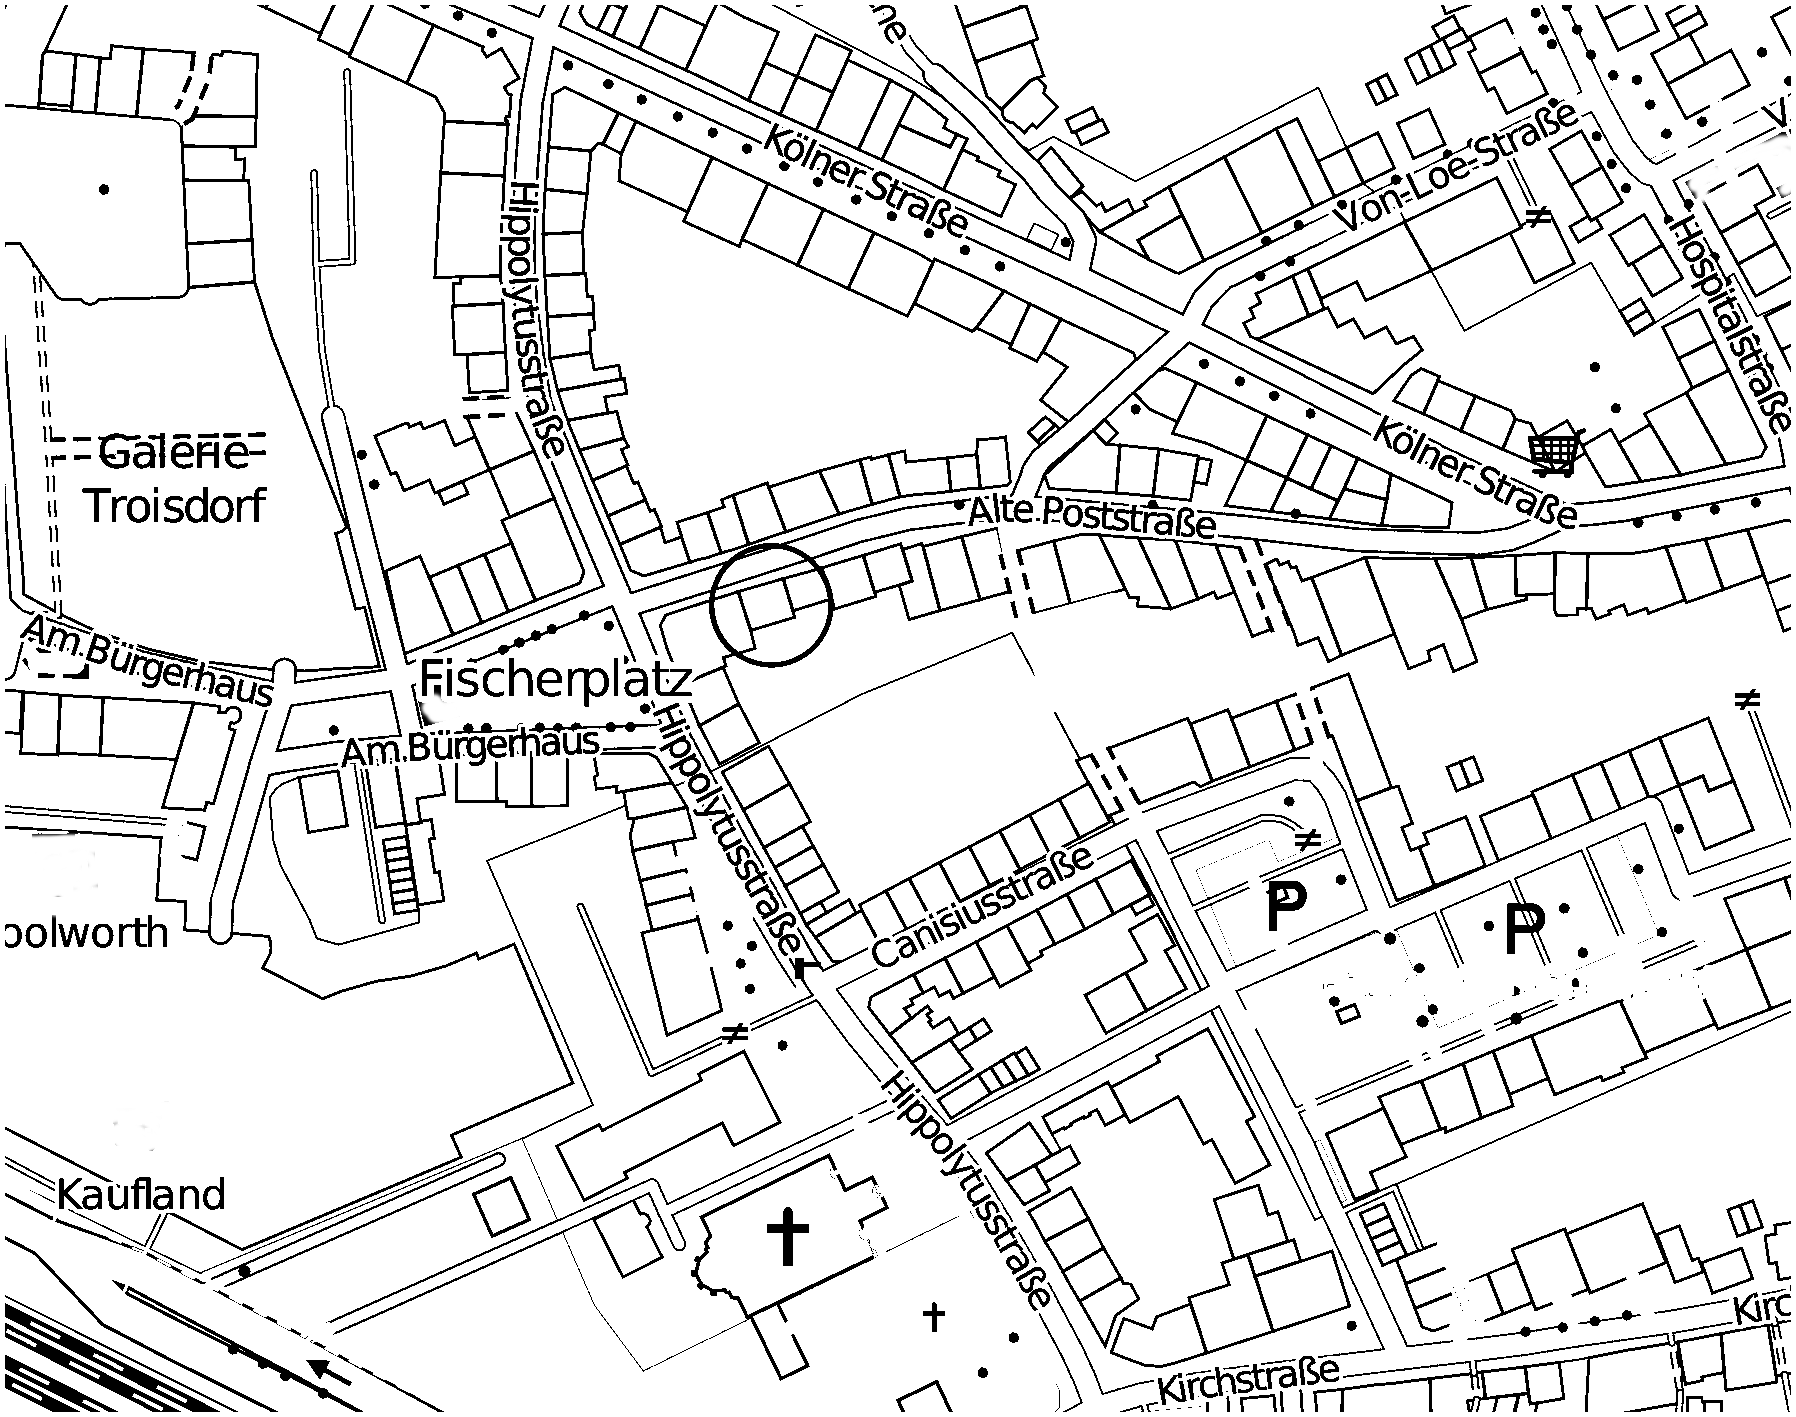
\includegraphics[width=\textwidth]{gfx/map/rect28239c}
\end{center}

\end{document}